\section{Introduction}
Game design is a difficult discipline that typically requires many years of experience to get right. An important aspect of game design is \textit{game feel}, i.e., the sensation of control in a videogame, as described by Swink \cite{swink}. Game feel is the extension of the player's senses. It's caused by a constant feedback loop between player and system. At its core, game feel can be described as the pure enjoyment of moving a player avatar\footnote{Merriam-Webster defines a computer avatar as \textit{a small picture that represents a computer user in a game, on the Internet, etc.} \cite{avatar}} around on the screen. Game feel happens from the moment players form an intention in their heads and press a button, to when they see the response on the screen (e.g., the avatar jumping). Whenever players interact with a game, they are exposed to the feel of that game. This means that the feel can make or break the player experience.

The current state of designing game feel is that of an iterative process wherein designers have to carefully consider and tweak every aspect to get the game feeling ``right". This process often relies on the gut feeling of the game designers, typically combined with extensive testing. There is little practical framework or vocabulary that designers can build upon.

Even though game feel is usually based on the simulation of a virtual world, it can still be related to the physical world. Every object in the physical world has properties that define their unique feel, e.g., their textures, shapes and interactive properties. While a bowling ball feels massive and heavy, a knife feels sharp, pointy and thin. When it comes to games, designers and players don't have the required vocabulary to talk about these characteristics. Game designers need to constantly make tiny adjustments in order to make their games feel good \cite{meatboy1, meatboy2, juicyBeast, platformer_controls, gameFeelTips}.

Players might describe a certain game feeling `floaty', `twitchy' or `responsive', but there are no de facto terms that can be used to talk about a specific game feel. It is uncertain when a game goes from being `twitchy' to `floaty'. Game feel consists of many elements, such as graphical presentation, physical simulations, sounds, player controls, input device, camera, level design, etc. It is difficult to isolate the influences of each of these aspects. Further research is needed in order to determine how much each of these elements affect the feel of a game --- and if these findings can be applied universally or only to specific game genres.

Even though game feel might be a loose concept, there are still the notion of responsiveness. West argued that \textit{``the `feel' of a game is, in large part, described in terms of how responsive it is. Very often a game will be described as `laggy' or `sluggish', and by contrast other games will be `tight' or `fast'."} \cite{measure_lag} However, these are somewhat loose terms. Therefore, this paper sets out to investigate two questions: A) What words players use to describe the feel of a game, and B) Which parameters yield those specific descriptions. This study is based on a simple 2D platforming game where players control a rolling ball with the keyboard. The acceleration and deceleration of the player's avatar change, separately, between rounds. To test the influence of changing these parameters, an experiment was conducted by uploading the game to the Internet. Participants had to play the same game four times, where each round changed the acceleration and deceleration. Between the rounds, they were asked to describe the feel of the controls in their own words, as well as rate it based on pre-defined terms such as how `twitchy', `fluid' and `stiff' the controls felt. 274 players participated in the experiment.
%and it is unclear when exactly a game goes from feeling `sluggish' to `tight'.

%This pattern is inspired by ADSR envelopes (Attack-Decay-Sustain-Release) \cite{adsr}, which are often used in order make an electronic musical instrument mimic the sound of a mechanical instrument, e.g., the sound of a pipe organ or a guitar string. This is achieved by modulating the amplitude over time.

This paper describes the background, setup and findings of the experiment. Section \ref{stateOfTheArt} describes the state of the art. Section \ref{design} presents a short description of the game that was developed for this project. Section \ref{experimentalDesign} describes the thoughts behind the experimental design. Section \ref{data} presents an analysis of the collected data, and, lastly, Section \ref{discussion} discusses and concludes upon this data.

\section{State of the Art} \label{stateOfTheArt}
Section \ref{define_GF} provides a definition of game feel and describes other relevant topics. Section \ref{colour} looks at a study about how people describe colours. This study has been used as inspiration for conducting the experiment about how people describe game feel. Section \ref{marioLevel} reviews a study that built a set of questionnaires directly into a game, which was then put online.

%This paper sets out to investigate one of these aspects, namely the influence of movement controls in 2D platforming games.

\subsection{Defining Game Feel} \label{define_GF}
Game feel is a relatively unexplored research area. The primary literature on the topic is the book \textit{Game Feel: A Game Designer's Guide to Virtual Sensation} by Swink \cite{swink}. `Feel' is not meant in a thematic nor emotional/physical sense. Instead it's the kinesthetic sense of manipulating a virtual object --- the sensation of real-time control in a videogame. Talking to game designers, Swink found that game feel is associated with intuitive controls, physical interactions with virtual objects (and the timing and impact of these interactions), as well as aesthetic pleasure and appeal in the form of polishing effects. Having analyzed various games and their components, Swink provided the following definition of game feel: \textit{real-time control of virtual objects in a simulated space, with interactions emphasized by polish} \cite{swink}. These elements will be discussed further in the following sections.

\subsection{Reacting to Player Input}
An important aspect of game feel is controlling virtual objects and how responsive these controls are. Normoyle and J\"{o}rg conducted a study to investigate the relationship between the naturalness of motion (e.g., in the form of realistic and adaptive 3D animations) versus responsiveness (the game reacts instantly to the player's input, regardless of which phase the animation is in) \cite{normoyle_trade-offs_2014}. Developers typically need to make trade-offs between naturalness and promptness when designing and implementing player controls and animations. This can affect the player's overall sense of control, enjoyment, satisfaction and performance. To test this, Normoyle and J\"{o}rg  created a 3D game with varying degrees of animation blendings. The more natural the animations blend together when moving, the less responsive the character is (e.g., the player has to wait for the virtual character to complete a ``turn-around" animation). While playing, 67 participants tried the different animation types.  Data was collected by logging the participants' performance in the game, as well as asking them about their experience via a post-questionnaire. Normoyle and J\"{o}rg concluded that one should always prioritize responsiveness, since low responsiveness negatively affects players' perceived ease of use, as well as their objective performances \cite{normoyle_trade-offs_2014}.

This knowledge can be tied into the Model Human Processor \cite{card1986model, swink}, implying that games should respond to the player's input within 240 milliseconds in order to appear instant. Swink describes feedback happening within 100 milliseconds as being `instant' and within 100-240 milliseconds as being `sluggish'. This perception is gradual, and if there is a delay of more than 240 milliseconds, the sense of real-time control is broken \cite{swink}. Also, the computer must provide feedback by displaying images at a rate greater than 10 frames per second in order to maintain the impression of motion.

How quickly the game reacts to player input is important. One way to measure this response lag is provided by West. He presented ways to measure this lag and how it can be minimized, by understanding the sequence of events that occur from the time the player presses a button, to when the results appear on the screen \cite{measure_lag, program_lag}. By using a high-speed camera (60 frames per second) to record both the input device (e.g., a controller) and the screen, it is possible to measure this latency \cite{euro}.

%\begin{figure}[htbp]
%\centering
%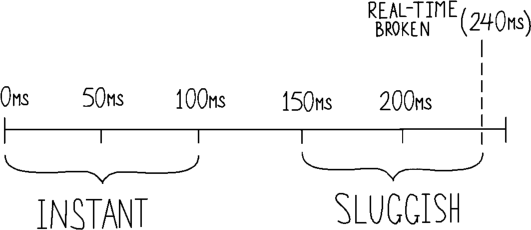
\includegraphics[width=0.30\textwidth]{Pics/response}
%\caption{Model of response time and player perception. Figure inspired by Swink \cite{swink}.}
%\label{fig:response}
%\end{figure}

%\subsubsection*{Intuitive and Clear Feedback}
West also provided a good overview of how to implement intuitive non-ambiguous controls in games, by measuring the player's input and comparing it to how the game responds \cite{intuitive_buttons}. An example of this is the ``ghost jump" \cite{ghostJump, canabalt}: players have reached the edge of a platform and decide to jump. However, according to the game's internal physical simulation, the players have already left the ground and are therefore not able to jump. Even though they perceived themselves to be on the ground when pressing the jump button, the game fails to meet this intention. This dissonance, between what the players perceived and what actually happened in the simulation, can have a negative effect on the game feel.
% --- in the end, it is the players' perception that matters.

%A good-feeling game should afford players whatever they want without having them to think too much about it.

\subsection{Enhancing Player Experience with Polishing Effects} \label{polishSection}
Polishing effects, including what some game designers call \textit{juiciness} \cite{juice3}, can be used to make a game's simulation feel more alive. Schell described juciness with the following words: \textit{``When a system shows a lot of second-order motion that a player can easily control, and that gives the player a lot of power and rewards, we say that it is a juicy system --- like a ripe peach, just a little bit of interaction with it gives you a continuous flow of delicious reward."} \cite{schell_art_2008} In other words, the system should give the player continuous feedback for their actions. Game designers Jonasson, Purho and Nijman demonstrated how simple games can feel better by adding layers of effects, such as bouncing motions, screen shake, particles, sounds, impact effects and fluid camera movements, to provide as much visual and auditory flair as possible \cite{juice1, juice2}. Berbece provided similar examples with animation effects \cite{animationSucks}. To some extent, this can be related to the 12 Basic Principles of Animation, which are techniques artists can use to make their animations come to life \cite{animation}. Based on personal experience, game designer Rogers proposed a list of related techniques that can be utilized in games, such as freezing the animation for a few frames to emphasize a great impact \cite{sticky}.

%On their GitHub page, \cite{juice1} wrote: \textit{``A juicy game feels alive and responds to everything you do tons of cascading action and response for minimal user input.} (\textit{sic})\textit{"} 

\subsection{Colour Naming} \label{colour}
Guest and Van Laar conducted an experiment to investigate how people describe colours \cite{guest_structure_2000}. Their approach, as well as how they categorize colours into different categories, has served as an inspiration for how to make participants describe game feel in this project

Among ten native English speakers, Guest and Van Laar collected three types of measurements: response times, confidence ratings and consistencies. These were later collapsed into one \textit{nameability} feature using principal components analysis, which described a single measure of ease of naming colours. The participants were seated in front of a computer and asked to name the colours on screen. It was stressed that the chosen names should be those that the participants would use to acceptably describe that colour to another person. Additionally, it was decided to not restrict the names that were allowed: participants could use unconstrained naming (`bright red') or monolexemic naming (using root words such as `red') as they preferred. After the experiment, a classification scheme was devised in order to assist the data analysis, by splitting names into one of eight categories, based on prior research in the area. These categories were:
\begin{itemize}[noitemsep,nolistsep]
\item Landmark basic (`red', `green', `blue', `yellow')
\item Other basic (`orange', `grey')
\item Other monolexemic (`peach', `lilac')
\item Basic-basic (`blue-green', `green-yellow')
\item Hue-modified basic (`sea green', `red peach')
\item Lightness-modified basic (`light green', `mid blue')
\item Lightness-modified monolexemic (`light peach', `dark turquoise')
\item Other [complex] (`bright sea green')
\end{itemize}
Guest and Van Laar found that despite the naming being unconstrained, the participants mainly used unmodified basic terms to describe the colours (such as `red', `green' and `blue'), as opposed to non-basic monolexemic names (such as `peach', `mauve', `violet' and `turquoise') and lightness-modified basic terms (such as `light blue' and `light green'). This suggests that basic terms might be enough to describe the main nuances of colours. However, Guest and Van Laar also stressed that there exists regions of the colour space that are especially hard to name.

\subsection{Collecting Data via the Internet} \label{marioLevel}
Pedersen, Togelius and Yannakakis set out to examine the relationship between level design parameters of platform games, individual playing characteristics and player experiences \cite{marioModel}. Their approach to collect data via the Internet has served as an inspiration for collecting data about game feel.

They constructed a computational model of players' experiences derived from gameplay interactions in a \textit{Super Mario Bros.}-styled game. The goal was to create a system that can automatically generate content tailored to the player experience according to the needs of the game design. A neural network model was used to map between level design parameters, player behaviour and player-reported emotions. The experiment focused on three types of data: controllable level design features (e.g., number of gaps and the spatial diversity of gaps), gameplay characteristics (e.g., number of jumps, time spent running and standing still) and the players' expressions of their experiences (e.g., comparing two levels against each other)

To obtain data, Pedersen, Togelius and Yannakakis uploaded their game as a Java applet on a website (additionally, they also provided a standalone download). Users were recruited via posts on blogs and mailing lists. A questionnaire was built into the game. Each participant played a pre-defined set of four games in pairs, where the levels differed in one or more of the four controllable level design parameters. For each completed pair of games, the players were asked to report their emotional preference in a questionnaire (see Figure \ref{fig:mario}). This method allowed them to collect data from 181 test participants. Pedersen, Togelius and Yannakakis found seven features that are significantly correlated with fun, as well as several features that can predict fun.

%; however, these don't include any challenging elements (cf. the theory of flow). They also found several features that can predict fun (three features: 69\%), challenge (five features: 77\%) and frustration (four features: 88\%), but cannot reliably predict fun from controllable level design features yet.

\begin{figure*}[htbp]
\centering
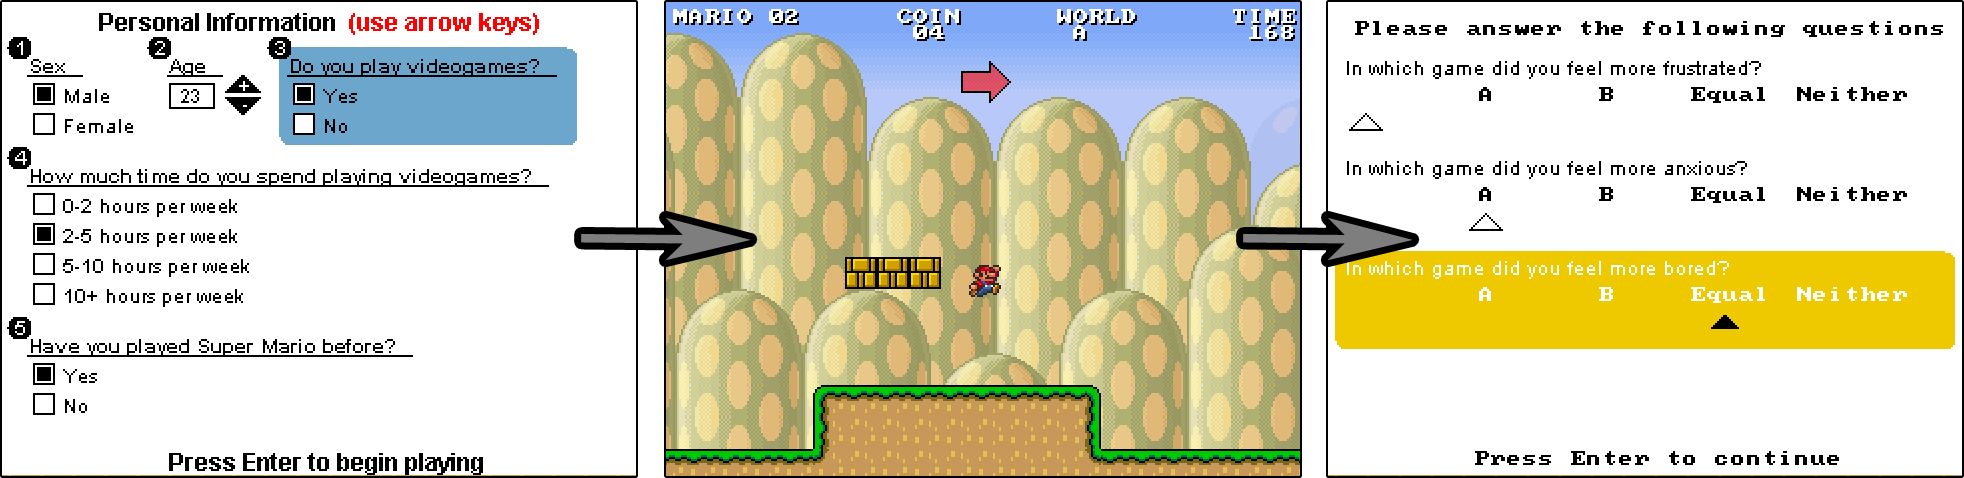
\includegraphics[width=0.95\textwidth]{Pics/mario_all2}
\caption{Using a Java web applet, Pedersen, Togelius and Yannakakis collected data about player preferences in level design, by building a questionnaire directly into the game. Figure inspired by \cite{marioModel}.}
\label{fig:mario}
\end{figure*}